\chapter{Vulnerability}
\label{ch:vulnerability}

\section{MMI conversion}

The vulnerability curves defined maps the relationship of a loss ratio to 
Modified Mercalli Intensity. The formula used to convert spectral acceleration 
to MMI is the formula from Atkinson and Kaka (2007), and is used for a period 
of 1 second. \\

\begin{equation} \label{eq:rsa_mmi}
MMI = 
\begin{cases}
C_1 + C_2 log Y	& \quad \mbox{if $log Y \le log Y(I5)$} \\
C_3 + C_4 log Y	& \quad \mbox{if $log Y \ge log Y(I5)$} \\
\end{cases}
\end{equation}

\begin{table}
\caption{Coefficients of equation \ref{eq:rsa_mmi} (EQRM uses PSA (1Hz))}
\begin{center}
\begin{tabular}{l c c c c c}
\hline
\hline
$Y$ & PGV & PGA & PSA (0.5 Hz) & PSA (1 Hz) & PSA (3.3 Hz) \\
\hline
$C_1$ & 4.37 & 2.65 & 3.72 & 3.23 & 2.40 \\
$C_2$ & 1.32 & 1.39 & 1.29 & 1.18 & 1.36 \\
$C_3$ & 3.54 & 1.91 & 1.99 & 0.57 & 1.83 \\
$C_4$ & 3.03 & 4.09 & 3.00 & 2.95 & 3.56 \\
$log Y(I5)$ & 0.48 & 1.69 & 1.00 & 1.50 & 1.92 \\
$\sigma_{1MMI}$ & 0.80 & 1.01 & 0.86 & 0.84 & 0.88 \\
\end{tabular}
\end{center}
\end{table}

\section{Determining mean loss and sigma}

Figure \ref{fig:fig-padang-curve} shows a graphical representation of a curve
dataset. For a given MMI level, mean loss and sigma can be determined by linearly 
interpolating the points in the curve. Numpy�s interp function provides an 
efficient way of doing this. e.g. for the NEL 1.4.1 curve, MMI = 9.0, \\

\begin{lstlisting}
>>> mean_loss = interp(9.0, MMI, NEL_141_lossratio)
>>> cv = interp(9.0, MMI, NEL_141_cv)
>>> sigma = cv*mean_loss
>>> mean_loss
0.790940996
>>> sigma
0.23728229879999999
\end{lstlisting}

\begin{figure}[htp]
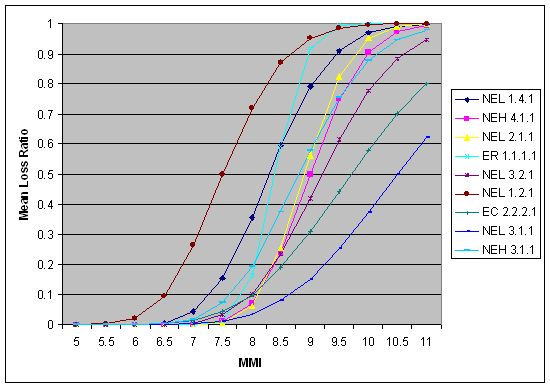
\includegraphics[scale=0.75]{fig-padang-curve}
\caption{Vulnerability curves based on data collected from Padang, Indonesia}
\label{fig:fig-padang-curve}
\end{figure}

\section{Probabilistic sampling}

EQRM uses the following method to sample the results from vulnerability curve 
interpolation \\

\begin{itemize}
\item Select a random number $n_{rand}$ from the standard normal distribution 
$N \sim (0,1)$
\item Compute $lossRatio$ as follows
\begin{equation}
lossRatio = meanLoss + n_{rand}\sigma
\end{equation} 
\end{itemize}

For each vulnerability function, a probabilistic distribution can be specified. 
EQRM supports lognormal and normal. If the function is lognormal, the 
exponential of the $lossRatio$ will be returned. \\
\\
This may return results outside the ratio boundary (0, 1). e.g for the above 
$meanLoss$ and $\sigma$ values using the distribution function in used in EQRM 
for sampling, \texttt{sample\_for\_eqrm},\\

\begin{lstlisting}
>>> dist.sample_for_eqrm(mean_loss, sigma)
0.73610087492782117
>>> dist.sample_for_eqrm(mean_loss, sigma)
0.61621877829645755
>>> dist.sample_for_eqrm(mean_loss, sigma)
0.78716766000165828
>>> dist.sample_for_eqrm(mean_loss, sigma)
0.80414262679118687
\end{lstlisting}

A cutoff will be applied:
\begin{itemize}
\item $lossRatio > 1 = 1$
\item $lossRatio < 0 = 0$
\end{itemize}

\section{Calculating loss}

Economic loss is the figure to be calculated per site. As the defined curve 
produces a single loss figure, contents loss cannot be estimated in this way. 
Economic loss is based on the following attributes of a site: \\

\begin{itemize}
\item \texttt{BUILDING\_COST\_DENSITY} ($bcd$)
\item \texttt{FLOOR\_AREA} ($fa$)
\item \texttt{SURVEY\_FACTOR} ($sf$)
\end{itemize}

This is calculated as

\begin{equation}
economicLoss = bcd \times fa \times sf \times lossRatio
\end{equation}
